\documentclass{beamer}
\usetheme{Madrid}
\usepackage{array}
\usepackage{tikz}
\usepackage{multicol}
\usepackage{amsmath}
\usepackage{mathtools}
\title[CST 301 M3]{FORMAL LANGUAGES AND AUTOMATA THEORY}
\subtitle{Module 3}
\author{Rijin IK}
\institute[VJEC]{Assistant Professor\\Department of Computer Science and Engineering\\Vimal Jyothi Engineering College\\Chemperi}
\begin{document}
	\begin{frame}
		\titlepage
	\end{frame}
   \begin{frame}{Outline}
   \tableofcontents
   \end{frame}
\section{Course Outcomes}
\begin{frame}{Course Outcomes}
\textbf{After the completion of the course the student will be able to}
\begin{enumerate}
	\item Classify a given formal language into Regular, Context-Free, Context
	Sensitive, Recursive or Recursively Enumerable. [Cognitive knowledge
	level: Understand]
	\item Explain a formal representation of a given regular language as a finite state
	automaton, regular grammar, regular expression and Myhill-Nerode
	relation. [Cognitive knowledge level: Understand]
	\item Design a Pushdown Automaton and a Context-Free Grammar for a given
	context-free language. [Cognitive knowledge level : Apply]
	\item Design Turing machines as language acceptors or transducers. [Cognitive
	knowledge level: Apply]
	\item Explain the notion of decidability. [Cognitive knowledge level:
	Understand]
\end{enumerate}
\end{frame}
\section{Myhill-Nerode Relations (MNR)}
\begin{frame}{Myhill-Nerode Relations (MNR)}
\textbf{Equivalence relation}
\begin{itemize}
	\item Let $R \subseteq \Sigma^*$ be a regular set, and let $M = (Q, \Sigma, \delta, q_0, F)$ be a DFA  for 
	R with no inaccessible  states. The automaton M induces an Equivalence 
	relation $\equiv_M$ on $\Sigma^*$ defined by
	$$x \equiv_M y \xLeftrightarrow{def} \hat{\delta}(q_0,x) = \hat{\delta}(q_0,y). $$
\end{itemize}
[Equivalence  relation$\rightarrow$ it is reflexive, symmetric, and transitive]
\begin{itemize}
	\item \textbf{Reflexive}
	\begin{itemize}
		\item $\forall_x \in\Sigma^*,\hat{\delta}(q_0,x)=\hat{\delta}(q_0,x)$
	\end{itemize}
\item \textbf{Symmetric}
\begin{itemize}
	\item $x\equiv_M y \implies \hat{\delta}(q_0,x)=\hat{\delta}(q_0,y)\implies\hat{\delta}(q_0,y)=\hat{\delta}(q_0,x) \implies y\equiv_M x$
\end{itemize}
\item \textbf{Transitive}
\begin{itemize}
	\item suppose $x \equiv_M y \ and \ y \equiv_M z \implies x\equiv_M z$
\end{itemize}
\end{itemize}
\end{frame}
\begin{frame}{Myhill-Nerode Relations (MNR)}
	\textbf{Myhill-Nerode Relations (MNR)}
	\begin{itemize}
		\item The Myhill-Nerode relation for a regular set $R \subseteq \Sigma^*$ is an equivalence relation $\equiv$ on $\Sigma^*$ that satisfies three key properties: 
		\begin{enumerate}
			\item  It is a right congruence: for any $x, y \in \Sigma^*$ and $a \in \Sigma $,
			\begin{itemize}
				\item 	$x \equiv_m y \implies xa \equiv_m ya;$
			\end{itemize}
			\item It refines $L(M)$: for any $x, y \in \Sigma*$
			\begin{itemize}
				\item $x \equiv_m y \implies (x \in L(M) \Leftrightarrow y \in L(M));$
				\item i.e whenever $x \& y$ are related either  $x \& y$ are in the language or both  $x \& y$ are not in the language.
			\end{itemize}
			\item It is of finite index; that is, it has only finitely many equivalence classes. 
			\begin{itemize}
				\item This is beause there is exactly one equivalence class
				${x \in \Sigma^*\big| \hat{\delta}(q_0,x)=q}$ corresponding to eaeh state q of M. 
			\end{itemize}
		\end{enumerate}
	\end{itemize}
\end{frame}
\begin{frame}{Myhill-Nerode Relations (MNR)}
	\begin{block}{Formal definition of Myhill-Nerod Relation (MN relation)}
		Let L be a language over an alphabet set $\Sigma$.Then, an MN relation $\equiv$ is an equivalence relation on $\Sigma^*$, which is a right congruence of finite index refining L.
	\end{block}
\textbf{Example:}
\begin{itemize}
	\item $L={x\in \{a}^* \big| 3\ divides\  |x|\}$
	\item $x\equiv y \Leftrightarrow |x| mod 3=|y| mod\  3$. Equivalence classes are:
	\begin{itemize}
		\item $[\epsilon]=\{a^i \big| i \mod 3 =0\}$
		\item $[a]=\{a^i \big| i \mod 3 =1\}$
			\item $[a^2]=\{a^i \big| i \mod 3 =2\}$
	\end{itemize}
\end{itemize}
\end{frame}	
\subsection{Conversion of DFA  to MNR}	
\begin{frame}{Conversion of DFA  to MNR}
	\begin{block}{Lemma}
	If a language L is regular, then there is a Myhill-Nerode relation on $\Sigma^*$ with
	respect to L
	\end{block}
\proofname \\

L is Regular $\implies$ $\exists$ a DFA M such that L=L(M)
\par Consider a binary relation $\equiv_M$ on $\Sigma^*$ induced by$ M=(Q,\Sigma , \delta , q_0,F ) ,$ defined as
\begin{eqnarray*}
\forall_{x,y} \in \Sigma^*, x\equiv_M y \Leftrightarrow \hat{\delta}(q_0,x)=\hat{\delta}(q_0,y)
\end{eqnarray*}
we proved that $\equiv_M$ is an MN relation
\end{frame}
\begin{frame}{Conversion of DFA  to MNR}
	\textbf{Q:}Show the equivalence classes of  Myhill Nerod relation for the language $L=\{x \in \{a\}^* \big| 3 \ divides \ |x|\} $.\\
	\textbf{Soln:}
	\\ DFA for the above language\\
	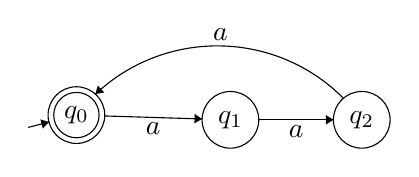
\begin{tikzpicture}[scale=0.12]
		\tikzstyle{every node}+=[inner sep=0pt]
		\draw [black] (22.4,-28.7) circle (3);
		\draw (22.4,-28.7) node {$q_0$};
		\draw [black] (22.4,-28.7) circle (2.4);
		\draw [black] (38.7,-29.2) circle (3);
		\draw (38.7,-29.2) node {$q_1$};
		\draw [black] (52.6,-29.2) circle (3);
		\draw (52.6,-29.2) node {$q_2$};
		\draw [black] (17.3,-30) -- (19.49,-29.44);
		\fill [black] (19.49,-29.44) -- (18.59,-29.15) -- (18.84,-30.12);
		\draw [black] (25.4,-28.79) -- (35.7,-29.11);
		\fill [black] (35.7,-29.11) -- (34.92,-28.58) -- (34.89,-29.58);
		\draw (30.53,-29.48) node [below] {$a$};
		\draw [black] (41.7,-29.2) -- (49.6,-29.2);
		\fill [black] (49.6,-29.2) -- (48.8,-28.7) -- (48.8,-29.7);
		\draw (45.65,-29.7) node [below] {$a$};
		\draw [black] (24.414,-26.481) arc (133.20471:44.89825:18.842);
		\fill [black] (24.41,-26.48) -- (25.34,-26.3) -- (24.66,-25.57);
		\draw (37.63,-20.86) node [above] {$a$};
	\end{tikzpicture}\\
The DFA has 3 states. so MNR partions the $\Sigma^*$ into 3 classes:
\begin{itemize}
	\item $C_1$=$\{x \in \Sigma^* \big | \hat{\delta}(q_0,x)=q_0\}$ $[q_0]=\{a^i \big| i \mod 3 =0\}$
	\begin{itemize}
		\item $c_1=\{\epsilon, a^3, a^6....\}$
	\end{itemize}
	\item  $C_2$=$\{x \in \Sigma^* \big | \hat{\delta}(q_0,x)=q_1\}$ $[q_1]=\{a^i \big| i \mod 3 =1\}$
		\begin{itemize}
		\item $c_2=\{ a^1, a^4....\}$
	\end{itemize}
	\item  $C_3$=$\{x \in \Sigma^* \big | \hat{\delta}(q_0,x)=q_2\}$ $[q_2]=\{a^i \big| i \mod 3 =2\}$
	\begin{itemize}
		\item $c_3=\{ a^2, a^5....\}$
	\end{itemize}
\end{itemize}
\end{frame}
\subsection{Conversion of MNR to DFA}	
\begin{frame}{Conversion of MNR to DFA}
	\textbf{Conversion of MNR to DFA}
	\begin{itemize}
		\item Given an MN relation $\equiv$ for a Language L over an alphabet set $\Sigma$, one can automatically construct a DFA $M_\equiv = (Q,\Sigma, \delta ,q_0,F)$, such that $L(M_\equiv)=L.$ 
		\begin{eqnarray*}
				Q &=&  \{[x] \big| x\in \Sigma^*\}\ \ set \ of \ all\ equivalent\  class \\
				q_0 &=& [\epsilon] \\
			\delta([x],a)&=&[xa] \\
			F&=& \{[x] \big| x\in L \}
		\end{eqnarray*}
		
	\end{itemize}
\end{frame}	
\begin{frame}{Conversion of MNR to DFA}
	\textbf{Example:}
	Consider the MN relation represented by the following equivalence  classes for the language : $L=\{x \in \{a\}^* \big| 3 \ divides \ |x|\} $.\\

Equivalence classes are:
\begin{itemize}
	\item $[\epsilon]=\{a^i \big| i \mod 3 =0\}$
	\item $[a]=\{a^i \big| i \mod 3 =1\}$
	\item $[a^2]=\{a^i \big| i \mod 3 =2\}$
\end{itemize}
\begin{multicols}{2}
\begin{eqnarray*}
	Q &=&  \{[x] \big| x\in \Sigma^*\} \\
	q_0 &=& [\epsilon] \\
	\delta([x],a)&=&[xa] \\
	F&=& \{[x] \big| x\in L \}
\end{eqnarray*}
	\columnbreak
	\begin{center}
		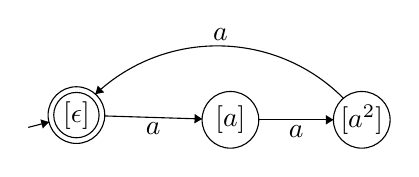
\begin{tikzpicture}[scale=0.12]
			\tikzstyle{every node}+=[inner sep=0pt]
			\draw [black] (22.4,-28.7) circle (3);
			\draw (22.4,-28.7) node {$[\epsilon]$};
			\draw [black] (22.4,-28.7) circle (2.4);
			\draw [black] (38.7,-29.2) circle (3);
			\draw (38.7,-29.2) node {$[a]$};
			\draw [black] (52.6,-29.2) circle (3);
			\draw (52.6,-29.2) node {$[a^2]$};
			\draw [black] (17.3,-30) -- (19.49,-29.44);
			\fill [black] (19.49,-29.44) -- (18.59,-29.15) -- (18.84,-30.12);
			\draw [black] (25.4,-28.79) -- (35.7,-29.11);
			\fill [black] (35.7,-29.11) -- (34.92,-28.58) -- (34.89,-29.58);
			\draw (30.53,-29.48) node [below] {$a$};
			\draw [black] (41.7,-29.2) -- (49.6,-29.2);
			\fill [black] (49.6,-29.2) -- (48.8,-28.7) -- (48.8,-29.7);
			\draw (45.65,-29.7) node [below] {$a$};
			\draw [black] (24.414,-26.481) arc (133.20471:44.89825:18.842);
			\fill [black] (24.41,-26.48) -- (25.34,-26.3) -- (24.66,-25.57);
			\draw (37.63,-20.86) node [above] {$a$};
		\end{tikzpicture}
	\end{center}
\end{multicols}
\end{frame}	
\section{Myhill-Nerode Theorem (MNT)}
\begin{frame}{The Myhill–Nerode Theorem}
	\textbf{The Myhill–Nerode Theorem}
	\begin{itemize}
		\item Let $R \subseteq \Sigma^*$. The following statements
		are equivalent:
		\begin{enumerate}
			\item R is regular;
			\item  There exists a Myhill-Nerode relation for R:
			\item The relation $\equiv_R$ is of finite index.
		\end{enumerate}
	\end{itemize}
\end{frame}	
\begin{frame}{The Myhill–Nerode Theorem}
	\textbf{Applications of MNT}
	\begin{itemize}
		\item Proving whether a language is regular or not.
		\item It can be also used to find the minimal number of states in a Deterministic Finite Automata (DFA).
	\end{itemize}
\end{frame}	
\begin{frame}{The Myhill–Nerode Theorem}
	\textbf{Example:}Is the following language regular
	$$L=\{x \in \{a,b\}^* \big| \mbox{number of a in x is odd}\}$$
	\textbf{Sln:}\\
	\begin{itemize}
		\item It is enough to prove that $\equiv_L$ is of finite index
		\item Recall that: $\forall_{x,y} \in \Sigma^*, x\equiv_L y\  iff\  \forall_z \in \Sigma^*, (xz\  \in L \ \Leftrightarrow yz \in L)$
		\item Equivalence classes of $\equiv_L:$
		\begin{itemize}
			\item Suppose $x,y,z \in \{a,b\}^*$ such that number of a in x is even and number of a in y is even:
			\item \textbf{Case 1:} number of a in z is odd
			\begin{eqnarray*}
				 &\implies &\mbox{ number of a in  (xz) is odd and number of a in  (yz) is odd}\\
				  &\implies & xz \in L \ and \ yz \in L
			\end{eqnarray*}
				\item \textbf{Case 2:} number of a in z is even
			\begin{eqnarray*}
				&\implies &\mbox{ number of a in  (xz) is even and number of a in  (yz) is even}\\
				&\implies & xz \notin L \ and \ yz \notin L
			\end{eqnarray*}
		so the equivalent class is $[\epsilon] = \{x \in \{a,b\}^* \big| \mbox{number of a in z is even}\}$ 
	
		\end{itemize}
		
	\end{itemize}
\end{frame}	
\begin{frame}{The Myhill–Nerode Theorem}
	\small
	\textbf{Sln cont..:}\\

		\begin{itemize}
			\item Suppose $x,y,z \in \{a,b\}^*$ such that number of a in x is  odd and number of a in y is  odd:
			\item \textbf{Case 1:} number of a in z is odd
			\begin{eqnarray*}
				&\implies &\mbox{ number of a in  (xz) is even and number of a in  (yz) is even}\\
				&\implies & xz \notin L \ and \ yz \notin L
			\end{eqnarray*}
			\item \textbf{Case 2:} number of a in z is even
			\begin{eqnarray*}
				&\implies &\mbox{ number of a in  (xz) is odd and number of a in  (yz) is odd}\\
				&\implies & xz \in L \ and \ yz \in L
			\end{eqnarray*}
			so the equivalent clas is $[a] = \{x \in \{a,b\}^* \big| \mbox{number of a in z is odd}\}$ 
			
		\end{itemize}
Equivalence classes of $\equiv_L:$
\begin{enumerate}
	\item $[\epsilon] = \{x \in \{a,b\}^* \big| \mbox{number of a in z is even}\}$ 
	\item $[a] = \{x \in \{a,b\}^* \big| \mbox{number of a in z is odd}\}$ 
\end{enumerate}
Thus $\equiv_L$ is of finite index and hence the language is regular
\end{frame}	
\section{Context Free Grammars}
\begin{frame}{Context Free Grammars}
	\textbf{Context Free Grammars}
	\begin{itemize}
		\item Context-free grammars (CFGs) are used to describe context-free languages.
		\item A context-free grammar is a set of recursive rules used to generate patterns of strings.
		\item A context-free grammar can describe all regular languages and more, but they cannot describe all possible languages.
		\begin{itemize}
			\item i.e It is\textbf{ more powerfull than Regular grammar }
		\end{itemize}
	\item Widely used in Programming Languages-syntax,parsing.
	\end{itemize}
\end{frame}
\begin{frame}{Context Free Grammars}
\textbf{Applications of Context Free Grammar (CFG)}
\begin{itemize}
	\item For defining programming languages
	\item For parsing the program by constructing syntax tree
	\item For translation of programming languages
	\item For describing arithmetic expressions
	\item For construction of compilers
	\item Document Type Definition in XML is a Context Free Grammars which describes the HTML tags and the rules to use the tags in a nested fashion.
\end{itemize}
\end{frame}
\begin{frame}{Context Free Grammars}
	\textbf{ Formal definition of Context Free Grammars}
	\begin{itemize}
		\item A context-free grammar (CFG) is denoted $G = (V, T, P, S)$, 
		where
		\begin{itemize}
			\item V and T are finite sets of variables and terminals, respectively.
			\item P is a finite set of productions; each production is of the form $A \rightarrow \alpha$,
			\begin{itemize}
				\item where A is a variable and $\alpha$ is a string of symbols from $(V \cup T)^*$.
			\end{itemize} 
			\item S is a special variable called the start symbol.
		\end{itemize}
	\end{itemize}
\end{frame}

\begin{frame}{Context Free Grammars}
	\textbf{Language generated by CFG}
	\begin{itemize}
		\item The notation $S \xRightarrow[G]{*}w$ represents the fact that we can derive the string w from the start symbol of the grammar G in zero or more steps
		\item 	The language generated by G [denoted $L(G)$]  is $\{w \big|\  w\  is\  in T^*\  and \ S \xRightarrow[G]{*}w \}.$
		That is, a string is in L(G) if:
		\begin{itemize}
			\item The string consists solely of terminals.
			\item The string can be derived from S.
		\end{itemize}
	\end{itemize}

	$^*$A language  A is said to be a context free language if there exsits a context free grammar G such that $A=L(G)$\\
	$^*$The production rules are context-independent, meaning the replacement of non-terminal symbols can occur without regard to the surrounding context.\\
	\textbf{C language is an example for Context Free Language.}
\end{frame}
\begin{frame}{Context Free Grammars}
	\textbf{Example:}
	\begin{itemize}
		\item Write CFG for the language $ L= \{a^n b^n \big| n\geq1\}$
	\end{itemize}
\begin{eqnarray*}
	L&=& \{ab, aabb, aaabbb, aaaabbbb, aaaaabbbbb, ………….\}\\
	G &=& (\{S\}, \{a, b\}, P, S)
\\
\end{eqnarray*}
P:
\begin{eqnarray*}
	 S &\rightarrow& aSb \big| ab\\
	&(Or)&\\
	S &\rightarrow& aSB\\
	S &\rightarrow& aB\\
	B &\rightarrow& b\\
\end{eqnarray*}
\end{frame}
\subsection{Proving correctness of CFGs}
\begin{frame}{Proving correctness of CFGs}
\textbf{Proving correctness of CFGs}
\begin{itemize}
	\item $L \subseteq L(G ):$ Every string in L can be generated by G.
	\item $L(G) \subseteq L:$ G only generate strings of L.
\end{itemize}
\end{frame}
\begin{frame}{Proving correctness of CFGs}
\textbf{	Example: }
\begin{eqnarray*}
		G &=& (V, \Sigma, S, P) \\
	V &=& \{S\} \\
	\Sigma &=& \{0, 1\}\\ 
	S &=& S \\
	P &=& \{S \rightarrow 0S1 | S1 | \epsilon\}\\ 
	&or&\\ 
	G&:& S \rightarrow 0S1 | S1 | \epsilon \\
\end{eqnarray*}
$L(G) = L$ where $L = \{ 0^i1^j\big|\big|i\leq j\}$  prove $L(G) = L?$
\end{frame}
\begin{frame}{Proving correctness of CFGs}
	\textbf{Proof: }Need to show that $L \subseteq L(G)$ and $L(G) \subseteq L.$\\
	$\Rightarrow$ Suppose $x \in L$. Must show x can be generated by G.\\
	Proof by induction on the length of $x, \big|x\big|$ .\\
	\textbf{Basis:}
	\begin{itemize}
		\item  $|x| = 0.$ Then $x = \epsilon$ and $S \rightarrow \epsilon$ is a rule in G.
	\end{itemize}
\textbf{Induction Hypothesis:}
\begin{itemize}
	\item Suppose all words in L shorter than x can be generated in the grammar 
	and that $x \notin \epsilon$.
	\item Need to show x can also be generated.
	 
\end{itemize}
\textbf{Induction Step:}  since $x \in L, x = 0^i1^j$
\begin{itemize}
	\item \textbf{Case 1:} $i = 0\  so\  x = 1^j= 1^{j-1}1 $
	\begin{itemize}
			\item Since $1^{j-1} \in L$ and $|1^{j-1}| < |x|, S\xRightarrow{*} 1^{j-1}$ by the I.H.
			\item Then use rule $S \rightarrow S1$ followed by the derivation $S \xRightarrow{x} 1^{j-1}$ to construct x.
			\item Therefore, $x \in L(G)$
	\end{itemize}

	
\end{itemize}

\end{frame}
\begin{frame}{Proving correctness of CFGs}
	\textbf{Proof cont.. }
	
		\begin{itemize}
			\item	\textbf{Case 2:} $i \neq 0\  so\  x = 0^i1^j $
			\begin{itemize}
				\item Then $x' = 0^{i-1}1^{j-1}\in L$ since $i-1 \leq j-1.$
				\item $|x'| < |x|$ so by the I.H., $x' \in L(G)$ and $S\xRightarrow{*} 0^{i-1}1^{j-1}$
				\item Then use rule $S \rightarrow 0S1$ followed by the derivation $S \xRightarrow{*} 0^{i-1}1^{j-1}$ to construct x. 
				\item Thus $S\xRightarrow{*} x\  so\  x \in L(G).$ 
			\end{itemize}
		\end{itemize}	
\textbf{$\Leftarrow$}Must show if $x \in L(G)\  the\  x\  \in L.$\\
Proof by induction on k, the number of steps in x's derivation.\\
\textbf{Basis:} 
\begin{itemize}
	\item 1 step $(S\Rightarrow \epsilon)$: Then $x = \epsilon$ and $x \in L.$ 
\end{itemize}
\textbf{Induction Hypothesis:}
\begin{itemize}
	\item  Assume every word in L(G) with a shorter derivation than x is in L.
	\item Either $x = 0w1\  or\  x = w1$ where $w \in L(G)$ and w can be derived from S in less than k steps;
	\begin{itemize}
		\item i.e. $S \xRightarrow{<k}w$
	\end{itemize}
\end{itemize}
\end{frame}
\begin{frame}{Proving correctness of CFGs}
	\textbf{Proof cont.. }
	
	\begin{itemize}
		\item	By I.H. we know $w \in L$ so it has at least as many 1's as 0's
		\item Then by applying either $S \rightarrow 0S1 \ or\  S \rightarrow S1$ followed by the derivation $S \xRightarrow{*}$ w we obtain x in the form $0^i1^j$	where we are only increasing the difference of 1's to 0's so $i \leq j$ and $x \in L.$
	\end{itemize}	
Therefore, $L(G) \subseteq L$ and $L \subseteq L(G)$ so $L = L(G).$
\end{frame}
\section{Derivation Trees and ambiguity}
\begin{frame}{Derivation Trees and ambiguity}
\textbf{$\epsilon$ –Productions}
\begin{itemize}
	\item A production of the form $A \rightarrow \epsilon$, where A is a variable, is called a null 	production or $\epsilon$ –Productions
\end{itemize}
\textbf{Unit Productions}
\begin{itemize}
	\item A production of the form $A \rightarrow B$ whose right-hand side consists of a single 
	variable is called a unit production. 
	\item All other productions, including those of the form $A \rightarrow a$ and $\epsilon$ -productions, 
	are nonunit productions.

\end{itemize}
\textbf{Recursive Productions}
\begin{itemize}
	\item If a production's left side occurs in right side
	\item $S\rightarrow aS$ (Directly recursive)
	\item $S\rightarrow aA, \ A\rightarrow b|bS$ (indirectly recursive)
\end{itemize}
\end{frame}
\begin{frame}{Derivation Trees and ambiguity}
	\textbf{Derivation}
	\begin{itemize}
		\item Derivation is the process of applying productions repeatedly to expand non-terminals in terms of terminals or non-terminals, until there are no more 
		non-terminals.
		\item A derivation can be either Leftmost derivation or Right most 
		derivation.

		
	\end{itemize}
\textbf{Leftmost derivation}
\begin{itemize}
	\item If at each step in a derivation a production is applied to the leftmost 
	variable, then the derivation is said to be leftmost.
	\item \textbf{Example:}
	\begin{itemize}
		\item Consider the grammar $G = (\{S, A\}, \{a, b\}, P, S),$ where P consists of 
		\begin{eqnarray*}
		S& \rightarrow &aAS | a \\
		A& \rightarrow &SbA|SS|ba\\
\end{eqnarray*}
\item The corresponding rightmost derivation is 
	\begin{eqnarray*}
S \implies aAS \implies aSbAS \implies aabAS \implies aabbaS \implies aabbaa.
\end{eqnarray*}
	\end{itemize}
\end{itemize}
\end{frame}
\begin{frame}{Derivation Trees and ambiguity}
	\textbf{Rightmost derivation:}
	\begin{itemize}
		\item A derivation in which the rightmost variable is replaced at each step is said 
		to be rightmost.
		\item \textbf{Example:}
		\begin{itemize}
			\item Consider the grammar $G = (\{S, A\}, \{a, b\}, P, S),$ where P consists of 
			\begin{eqnarray*}
				S& \rightarrow &aAS | a \\
				A& \rightarrow &SbA|SS|ba\\
			\end{eqnarray*}
			\item The corresponding rightmost derivation is 
			\begin{eqnarray*}
				S \implies aAS \implies aAa \implies aSbAa \implies aSbbaa \implies aabbaa.
			\end{eqnarray*}
		\end{itemize}
	\end{itemize}
$^*$\textbf{Note:}“If w is in L(G) for CFG G, then w has at least one parse tree, and 
corresponding to a particular parse tree, w has a unique leftmost and a 
unique rightmost derivation.”

\end{frame}
\begin{frame}{Context Free Grammars}
	\textbf{Sentential Form:}
	\begin{itemize}
		\item A sentential form is any string consisting of non-terminals and/or terminals that is derived from a start symbol. 
		\item A string of terminals and variables $\alpha$ is called a sentential form if $S\xRightarrow{*}\alpha$
	\end{itemize}
\textbf{Example:}
\begin{itemize}
	\item Consider the grammar $G = (\{S, A\}, \{a, b\}, P, S),$ where P consists of 
	\begin{eqnarray*}
		S& \rightarrow &aAS | a \\
		A& \rightarrow &SbA|SS|ba\\
	\end{eqnarray*}
	\item The corresponding rightmost derivation is 

		$S \implies aAS \implies aAa \implies aSbAa \implies aSbbaa \implies aabbaa.$

\end{itemize}

$	S \xRightarrow{*} aAa$ ,	$S  \xRightarrow{*} aSbAa$,
$S\xRightarrow{*} aSbbaa$,$S\xRightarrow{*}aabbaa.$ are Sentential Form

\end{frame}
\subsection{Derivation Trees (or) Parse tree:}
\begin{frame}{Derivation Trees (or) Parse tree:}
\textbf{Derivation Trees (or) Parse tree:}
\begin{itemize}
	\item The derivations in a CFG can be represented using trees. Such trees 
	representing derivations are called derivation trees.

	\item Let G = (V, T, P, S) be a CFG. A tree is a derivation (or parse) tree for G if:
	\begin{enumerate}
	 \item Every vertex has a label, which is a symbol of $V \cup T \cup \{\epsilon \}$.
		\item The label of the root is S(start symbol).
		\item If a vertex is interior and has label A, then A must be in V.
		\item If n has label A and vertices $n_1, n_2, n_3, ..., n_k$ are the sons of vertex 	n, in order from the left, with labels $X_1, X_2, ......., X_k,$ respectively, 
		then $A \rightarrow X_1X_2 .......X_k$ must be a production in P.
		\item If vertex n has label $\epsilon$, then n is a leaf and is the only son of its father.

	\end{enumerate}
\end{itemize}
\end{frame}
\begin{frame}{Derivation Trees (or) Parse tree:}
	\small
Consider the grammar $G = (\{S, A\}, \{a, b\}, P, S),$ where P consists of
	\begin{eqnarray*}
		S  &\rightarrow& aAS | a\\
		A &\rightarrow&  SbA|SS|ba\\
	\end{eqnarray*}
	Construct a derivation tree for the string “aabbaa”
	\begin{figure}
		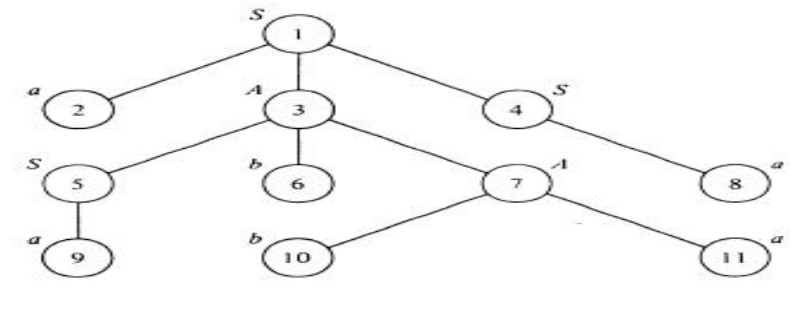
\includegraphics[scale=.3]{img3/m1}
		\caption{Derivation tree}
	\end{figure}
$S \implies aAS \implies aSbAS \implies aabAS \implies aabbaS \implies aabbaa.$\\
\textbf{Yield of a Tree:}The final string obtained by concatenating the labels of the leaves of the tree from left to right, ignoring the Nulls.(eg:-$aabbaa.$)
\end{frame}
\begin{frame}{Ambiguity in context free grammars:}
\textbf{Ambiguity in context free grammars:}
\begin{itemize}
	\item A context-free grammar G is said to be ambiguous if it has two parse trees
	for some word.
	\begin{center}
		(or)
	\end{center}
	\item A word which has more than one leftmost derivation or more than one 
	rightmost derivation is said to be ambiguous.

\end{itemize}
$^*$Note: A CFL for which every CFG is ambiguous is said to be an inherently 
ambiguous CFL\\

\end{frame}
\begin{frame}{Ambiguity in context free grammars:}
	\textbf{Example:}
	\begin{itemize}
		\item $G = (\{S\}, \{a, b, +, *\}, P. S),$ where P consists of $S\rightarrow S+S | S*S | a | b$ We have two derivation trees for $a + a * b$
	\end{itemize}
	\begin{figure}
		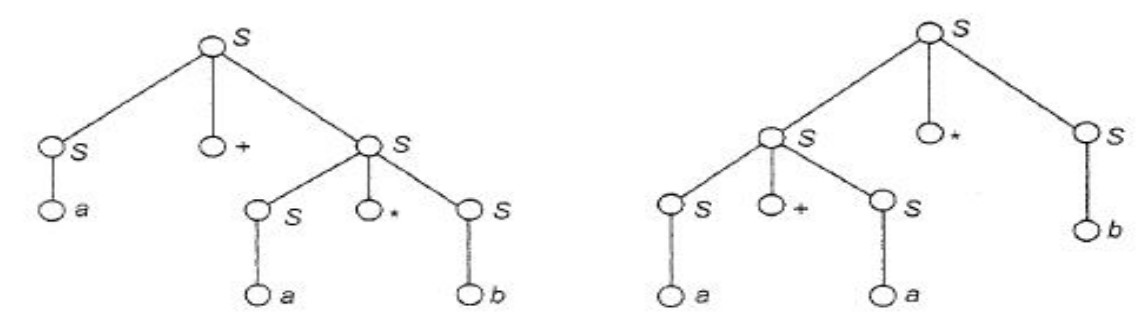
\includegraphics[scale=.5]{img3/m2}
		\caption{Two derivation trees for $a + a * b$}
	\end{figure}
\end{frame}
\begin{frame}{Simplified Context free grammar}
	\textbf{Reduction of context free grammar}
\begin{enumerate}
	\item We must eliminate useless symbol
	\begin{itemize}
		\item Eliminate non generating symbols
		\item Eliminate non reachable symbols
		
	\end{itemize}
	\item We must eliminate $\epsilon$-production
	\item We must eliminate Unit production
\end{enumerate}
\end{frame}



\begin{frame}{Simplified Context free grammar}
	\textbf{Eliminating useless symbol}
	\begin{itemize}
		\item Those variables or terminals that do not appears in any derivation of a terminal string from the start symbol
		\item A symbol $\gamma$ in CFG is usefull if and ony if 
		\begin{enumerate}
			\item $\gamma \xRightarrow{*}w$ where $w\in L(G)$ and $w\in T^*$ that is $\gamma$ leads to a string of terminals.
			 Here $\gamma$ is said to be generating.
			 \item If there is a derivation $S\xRightarrow{*} \alpha \gamma \beta \xRightarrow{*} w$ and $w \in L(G)$, for some $\alpha$ and $\beta$ then $\gamma$ is said to be reachable. 
	 		\end{enumerate}
 		\item So first eliminate symbols that are not generating and then eliminate  those symbols are not reachable.
	\end{itemize}
\end{frame}

\begin{frame}{Simplified Context free grammar}
	\textbf{Useful symbol}
	\begin{itemize}
		\item A symbol X in a CFG $G = \{V, T, P, S\}$ is called useful if there exist a
		derviation of a terminal string from S where X appears somewhere, else it is
		called useless.
		\begin{itemize}
			\item A symbol X is called generating if some terminal string can be dervied from	X.
			\item  A symbol X is called reachable if it can be reached from S.

		\end{itemize}
	\end{itemize}
\end{frame}


\begin{frame}{Simplified Context free grammar}
	\textbf{Example:}
	\begin{eqnarray*}
		S&\rightarrow& AB/a\\
		A&\rightarrow& b\\
	\end{eqnarray*}
\textbf{Solution:}
\begin{itemize}
	\item Identify nongenerating Symbol
	\item $S\rightarrow AB/a$ here B is nongenerating.
	\item The CFG become
		\begin{eqnarray*}
		S&\rightarrow& a\\
		A&\rightarrow& b\\
	\end{eqnarray*}
\item A is non reachable
\item The CFG become
\begin{eqnarray*}
	S&\rightarrow& a\\
\end{eqnarray*}
\end{itemize}
\end{frame}
\begin{frame}{Simplified Context free grammar}
	\textbf{Eliminate $\epsilon$-production}
	\begin{itemize}
		\item $\epsilon$-production are those productions that are of the form $X\rightarrow \epsilon $ these are also called null production
		\item A variable that derive $\epsilon$ ($A \xRightarrow{*} \epsilon)$  then we say A is nullable
		\item IN CFG, if there is $\epsilon$- production we can remove it without changing the meaning of the grammar.
		\begin{itemize}
			\item If $A\rightarrow \epsilon$ is a production to be eliminated then we look all production whose right side contain A
			\item And replace each occurence of A in each of these productions to obtain the non $\epsilon$-Productions.
			\item Now these resultant non $\epsilon$ -Production must be added to the grammar to keep the language generated the same.
		\end{itemize}
	\end{itemize}	
\end{frame}

\begin{frame}{Simplified Context free grammar}
	\begin{itemize}
		\item \textbf{Example:}
		\begin{eqnarray*}
			S&\rightarrow& aA\\
			A&\rightarrow& b|\epsilon\\
		\end{eqnarray*}
\item	$A\rightarrow\epsilon	$ is the $\epsilon$-production
\item Only one production $S\rightarrow aA$ whose right side contain A , so replace A by $\epsilon$
\item we get $S\rightarrow a$
\item add this new production to keep the language generated by this grammar same
\begin{eqnarray*}
	S&\rightarrow& aA\\
	S&\rightarrow& a\\
	A&\rightarrow& b\\
\end{eqnarray*}
	\end{itemize}	
\end{frame}
\begin{frame}{Simplified Context free grammar}
	\textbf{Eliminate Unit production}
	\begin{itemize}
		\item A production i of the form $A\rightarrow B$ is called unit production
		\item It increase the cost of derivation in a grammar
		\item If there exist  unit production in the grammar
		\begin{itemize}
			\item Select a unit production $A\rightarrow B$ such that there exist a production $B\rightarrow \alpha$ where $\alpha$ is a terminal
			\begin{itemize}
			\item For every nonunitproduction $B\rightarrow \alpha$
			\item Add production $A\rightarrow \alpha$ to the grammar
			\item Eliminate $A\rightarrow B$ from the grammar
		\end{itemize}
		\end{itemize}
	\end{itemize}	
\end{frame}
\begin{frame}{Simplified Context free grammar}
	\textbf{Example:}
	\begin{eqnarray*}
		S&\rightarrow& AB\\
		A&\rightarrow& a\\
		B&\rightarrow&C|b\\
		C&\rightarrow&D\\
		D&\rightarrow&E\\
		E&\rightarrow&a
	\end{eqnarray*}
\textbf{Solution}\\
Unit Productions are
\begin{eqnarray*}
	B&\rightarrow&C\\
	C&\rightarrow&D\\
	D&\rightarrow&E\\
\end{eqnarray*}
\end{frame}
\begin{frame}{Simplified Context free grammar}
\begin{itemize}
	\item Remove unit production $B\rightarrow C$ if there exists a production whose left side has C and right side contain a terminal but there is no such production in G,
	\item Similar things hold for production $C\rightarrow D$.
	\item Now we try to remove Unit production $D\rightarrow E$, because there is a production $E \rightarrow a$
	\item Eliminate $D\rightarrow E$ and introduce $D\rightarrow a$
	\item Grammar becomes
	\begin{eqnarray*}
		S&\rightarrow& AB\\
		A&\rightarrow& a\\
		B&\rightarrow&C|b\\
		C&\rightarrow&D\\
		D&\rightarrow&a\\
		E&\rightarrow&a
	\end{eqnarray*}
\end{itemize}
\end{frame}
\begin{frame}{Simplified Context free grammar}
	\small
	\begin{itemize}
		\item Now we can remove $C\rightarrow D$ by using $D\rightarrow a$ 
		\begin{eqnarray*}
			S&\rightarrow& AB\\
			A&\rightarrow& a\\
			B&\rightarrow&C|b\\
			C&\rightarrow&a\\
			D&\rightarrow&a\\
			E&\rightarrow&a
		\end{eqnarray*}
Similarly remove $B\rightarrow C$ by using $C\rightarrow a$ 
\begin{eqnarray*}
	S&\rightarrow& AB\\
	A&\rightarrow& a\\
	B&\rightarrow&a|b\\
	C&\rightarrow&a\\
	D&\rightarrow&a\\
	E&\rightarrow&a
\end{eqnarray*}
	\end{itemize}
\end{frame}
\begin{frame}{Simplified Context free grammar}
	\small
	\begin{itemize}
		\item 	$C\rightarrow a,	D\rightarrow a,	E\rightarrow a $ are useless symbols so the CFG become
		\begin{eqnarray*}
			S&\rightarrow& AB\\
			A&\rightarrow& a\\
			B&\rightarrow&a|b\\
		\end{eqnarray*}
	\end{itemize}
\end{frame}
\section{Chomsky Normal Form( CNF)}
\begin{frame}{Chomsky Normal Form( CNF)}
\textbf{Chomsky Normal Form( CNF)}
\begin{itemize}
	\item Any context-free language without $\epsilon$ is generated by a grammar in which all 
	productions are of the form $ A\rightarrow BC$ or$ A\rightarrow  a$. \item Here, A, B, and C, are variables 
	and a is a terminal.
\end{itemize}
\textbf{Converting CFG into CNF}
\begin{enumerate}
	\item Arrange that all bodies of length 2 or more consist only of variable
	\item Break bodies of length $\geq 3$ into cascade of productions each with a body consisting of two variables.
\end{enumerate}
\end{frame}
\begin{frame}{Chomsky Normal Form( CNF)}
Steps for converting CFG into CNF\\
	\textbf{Step 2:}Simplify the grammar.
	\begin{enumerate}[a]
		\item Eliminate $\epsilon$ –productions
		\item Eliminate unit productions
		\item Eliminate Useless symbols.
	\end{enumerate}
\end{frame}
\begin{frame}{Chomsky Normal Form( CNF)}
	\textbf{Step 3:}Eliminate terminals from RHS if they exist with other terminals or non-terminals.
	\begin{itemize}
		\item Consider a production in P,of the form $A\rightarrow X_1X_2X_3.....X_m$ where 
		$m\geq2$.If $X_i$ is a terminal,
		\item Introduce a new variable Ca and a production $C_a\rightarrow a$.
		\item Then replace $X_i$ by $C_a$. 
	\end{itemize}
	\textbf{Step 4:}
\begin{itemize}
	\item Consider a production $A\rightarrow B_1B_2B_3.....B_m$ where $m\geq3$,
	\item Create new 
	variables $D_1,D_2,....D_{m-2}$ and replace $A\rightarrow B_1B_2B_3...B_m$ by the set of productions 
	$\{A\rightarrow B_1D_1,D_1\rightarrow B_2D_2,..........D_{m-3}\rightarrow B_m-2 D_{m-2},D_{m-2}\rightarrow B_{m-1}B_m \}$
	
\end{itemize}
\end{frame}
\begin{frame}{Chomsky Normal Form( CNF)}
	\textbf{Example:}
	Consider the grammar $(\{S, A, B\}, \{a, b\}, P, S)$ that has the productions:
\begin{eqnarray*}
		S &\rightarrow&  bA | aB \\
		A &\rightarrow& bAA | aS | a\\
		B &\rightarrow&  aBB | bS | b\\
\end{eqnarray*}
\textbf{Sln:}\\
Step 1: Simplify the grammar.
\begin{itemize}
	\item The given grammar does not contain $\epsilon$ –productions, unit productions and 
	useless symbols. 
	\item It is in optimized form.
\end{itemize}
\end{frame}
\begin{frame}{Chomsky Normal Form( CNF)}
Step 2: 
\begin{itemize}
	\item The only productions already in proper form are $A\rightarrow  a$ and $B\rightarrow b.$
	\item So we may begin by replacing terminals on the right by variables, except in 
	the case of the productions $A \rightarrow  a$ and $B \rightarrow  b.$ 
	\item $S \rightarrow  bA$ is replaced by $S\rightarrow  C_bA$ and $C_b\rightarrow  b.$ 
	\item Similarly, $A\rightarrow  aS$ is replaced by $A \rightarrow  C_aS$ and $C_a\rightarrow  a$; $A\rightarrow  bAA$ is replaced by 
	$A\rightarrow C_bAA; S\rightarrow  aB$ is replaced by $S\rightarrow C_aB;
	B\rightarrow bS$ is replaced by $B\rightarrow  C_bS,$ and $B \rightarrow  aBB$ is replaced by $B\rightarrow  C_aBB.$
	
\end{itemize}
Step 3: 
\begin{itemize}
	\item In the next stage, the production $A\rightarrow C_bAA$ is replaced by $A \rightarrow  C_bD1$ and $D1\rightarrow AA,$ and the production $B\rightarrow C_aBB$ is replaced by $B\rightarrow  C_aD2$ and $D2 \rightarrow BB.
$
\end{itemize}

\end{frame}
\begin{frame}{Chomsky Normal Form( CNF)}
	The productions for the grammar in CNF are :
	\begin{eqnarray*}
		S&\rightarrow& C_bA | C_aB \\
		A &\rightarrow& C_aS | C_bD_1 | a\\
		B&\rightarrow& C_bS | C_aD_2 | b \\
		C_b&\rightarrow& b\\
		D1 &\rightarrow& AA \\
		D2 &\rightarrow& BB\\
		Ca&\rightarrow&  a\\
		Cb&\rightarrow&  b\\
	\end{eqnarray*}
\end{frame}
\section{Greibach Normal Form(GNF)}
\begin{frame}{Normal Form}
	\textbf{Left Recursion}
	\begin{itemize}
		\item A grammar which is of the form $A\rightarrow A \alpha|\beta$
		\item To avoid left recursion
		\begin{eqnarray*}
			A&\rightarrow& \beta A'\\
			A'&\rightarrow& \alpha A'\\
			A'&\rightarrow& \epsilon\\
		\end{eqnarray*}
	\item After removing $\epsilon$ production the grammar become
	\begin{eqnarray*}
			A&\rightarrow& \beta \big | \beta A'\\
		A'&\rightarrow& \alpha \big | \alpha A'\\
	\end{eqnarray*}
	\end{itemize}
\end{frame}
\begin{frame}{Greibach Normal Form(GNF)}
	\textbf{Greibach Normal Form(GNF)}
	\begin{itemize}
		\item Every context free language L without $\epsilon$ can be generated by a grammar for which every production is of the form $A\rightarrow a\alpha$ or $A\rightarrow a$
		\item Where A is a variable , a is a terminal and $\alpha$ is a string of variables.
	\end{itemize}
To convert given grammar into GNF following Two lemma's are considered\\
\textbf{Lemma1:}
\begin{itemize}
	\item Define an A-production to be a production with variable A on the left. 
	\item Let $G = (V, T, P, S)$ be a CFG. Let $A \rightarrow  \alpha_1B\alpha_2$ be a production in P and 
	$B\rightarrow \beta_1 | \beta_2|....|\beta_r$ be the set of all B-productions.
	\item Let $G1 = (V, T, P1, S)$ 
	be obtained from G by deleting the production $A \rightarrow  \alpha_1B\alpha_2$ from P and 
	adding the productions $A\rightarrow  \alpha_1\beta_1\alpha_2 | \alpha_1\beta_2\alpha_2 |...| \alpha_1\beta_r\alpha_2.$
	\item Then $L(G) = 	L(G1).$
\end{itemize}
\end{frame}
\begin{frame}{Greibach Normal Form(GNF)}
	\textbf{Lemma2:}
	\begin{itemize}
		\item Let $G = (V, T, P, S)$ be a CFG. Let $A\rightarrow A\alpha_1 | A\alpha_2 |...| A\alpha_r$ be
		the set of A-productions for which A is the leftmost symbol of the right-hand 
		side.
		\item Let $A \rightarrow  \beta_1 | \beta_2|...|\beta_s$ be the remaining A-productions. 
		\item Let $G1 = (V\cup \{B\}, T, P1, S)$ be the CFG formed by adding the variable B to V and 	replacing all the A-productions by the productions:

		\begin{multicols}{2}
			\begin{equation*}
				\left.\begin{aligned}
					A &\rightarrow& \beta_i\\
					A &\rightarrow& \beta_iB\\
				\end{aligned}\right\}  1\leq i \leq s
			\end{equation*}
							
			\columnbreak
			\begin{equation*}
			\left.\begin{aligned}
				B &\rightarrow& \alpha_i\\
				B &\rightarrow& \alpha_iB\\
			\end{aligned}\right\}  1\leq i \leq r
		\end{equation*}
		\end{multicols}
	\item Then $L(G1) = L(G).$
	\end{itemize}
\end{frame}

\begin{frame}{Greibach Normal Form(GNF)}
	\textbf{Algorithm for converting a CFG into GNF}
	\begin{enumerate}
		\item Remove Unit productions, useless symbols and $\epsilon$-production, if any.
		\item  For every terminal symbol  introduce a new non terminal. 
		\begin{itemize}
			\item $A \rightarrow Ba$ become $A \rightarrow BC_a, C_a\rightarrow a$
		\end{itemize}
		\item Introduce an order among nonterminals by renaming them.
		\item Using substitutions, rewrite productions (except Left Recursive) if required, to ensure that all productions of the form $X_i\rightarrow X_j\alpha$ satisfy the condition $i<j$
		\item Remove Left Recursions, if any.
		\item Remove unit productions,useless symbol if any added in step 4.
		\item Obtain the CFG in GNF by applying substitutions.
	\end{enumerate}
\end{frame}
\begin{frame}{Greibach Normal Form(GNF)}
	\textbf{Example:}Convert the following grammar into GNF
	\begin{eqnarray*}
		S&\rightarrow& AB|CC \\
		C&\rightarrow& b|SC \\
		A&\rightarrow&  a\\
		B&\rightarrow& b
	\end{eqnarray*}
	\textbf{Sln:}
	\begin{itemize}
		\item The given CFG is in CNF
		\item Renaming the nonterminals in G with index values
		\begin{itemize}
			\item Replace, S with $X_1$,A with $X_2$ ,B with $X_3$,C with $X_4$
		\end{itemize}
	\item Equivalent CFG G'
	\begin{eqnarray*}
		X_1&\rightarrow& X_2X_3|X_4X_4 \\
		X_4&\rightarrow& b|X_1X_4 \\
		X_2&\rightarrow&  a\\
		X_3&\rightarrow& b\\
	\end{eqnarray*}
	\end{itemize}
\end{frame}
\begin{frame}{Greibach Normal Form(GNF)}
	\textbf{Example cont..}
	\begin{itemize}
		\item The production $	X_4\rightarrow X_1X_4$ does not satisfy our requirement we need $i < j $
		\item Now, substitute the value of $X_1$ in $X_4$ we will get $X_4 \rightarrow X_2X_3X_4 \big| X_4X_4X_4$ 
		\item Substitute $X_2 \rightarrow a$ into   $X_4 \rightarrow X_2X_3X_4$ then $X_4 \rightarrow aX_3X_4$
		\item The production $X_4 \rightarrow  X_4X_4X_4$ is left recursive remove the leftrecursive 
		\item the grammar become
		\begin{eqnarray*}
			X_1&\rightarrow& X_2X_3|X_4X_4 \\
			X_4&\rightarrow& b|aX_3X_4|bX_5|aX_3X_4X_5 \\
			X_2&\rightarrow&  a\\
			X_3&\rightarrow& b\\
			X_5&\rightarrow& X_4X_4|X_4X_4X_5\\
		\end{eqnarray*}
	\end{itemize}
\end{frame}
\begin{frame}{Greibach Normal Form(GNF)}
	\textbf{Example cont..}
	\begin{itemize}
		\item Againg perform substitution then the grammar become
		\begin{eqnarray*}
			X_1&\rightarrow& aX_3|X_4X_4 \\
			X_4&\rightarrow& b|aX_3X_4|bX_5|aX_3X_4X_5 \\
			X_2&\rightarrow&  a\\
			X_3&\rightarrow& b\\
			X_5&\rightarrow& X_4X_4|X_4X_4X_5\\
		\end{eqnarray*}
	\end{itemize}
\begin{itemize}
	\item Againg substitute the value of $X_4$ then the grammar become
	\begin{eqnarray*}
		X_1&\rightarrow& aX_3|bX_4|aX_3X_4X_4|bX_5X_4|aX_3X_4X_5X_4 \\
		X_4&\rightarrow& b|aX_3X_4|bX_5|aX_3X_4X_5 \\
		X_2&\rightarrow&  a\\
		X_3&\rightarrow& b\\
		X_5&\rightarrow& X_4X_4|X_4X_4X_5\\
	\end{eqnarray*}
\end{itemize}
\end{frame}
\begin{frame}{Greibach Normal Form(GNF)}
	\textbf{Example cont..}
	\begin{itemize}
		\item Againg substitute the value of $X_4$ then the grammar become
		\begin{eqnarray*}
			X_1&\rightarrow& aX_3|bX_4|aX_3X_4X_4|bX_5X_4|aX_3X_4X_5X_4 \\
			X_4&\rightarrow& b|aX_3X_4|bX_5|aX_3X_4X_5 \\
			X_2&\rightarrow&  a\\
			X_3&\rightarrow& b\\
			X_5&\rightarrow& bX_4|aX_3X_4X_4|bX_5X_4|aX_3X_4X_5X_4|\\
			& &bX_4X_3|aX_3X_4X_4X_5|bX_3X_4X_5|aX_3X_4X_5X_4X_5\\
		\end{eqnarray*}
	\end{itemize}
\end{frame}
\end{document}